\chapter{Technologiewahl}
Im Kapitel der Technologiewahl werden einige aktuell erhältliche Smartwatch Modelle mit den theoretischen Daten verglichen, allgemeine Eigenschaften aufgeführt und die Entwicklerfreundlichkeit bewertet. Aufgrund der Bewertung von aufgestellten Kriterien werden für die Arbeit ein bis zwei Uhren ausgewählt.

\section{Allgemeine Eigenschaften}
Heute (Januar 2016) sind weitgehend alle erhältlichen tragbaren Computer am Handgelenk vom Smartphone abhängig (vgl. \cite{stwt:sw}). Deshalb bieten sie nur einen kleinen Mehrwert. Sie können zwar viel mehr als nur die Zeit anzeigen, jedoch sehr beschränkt und zum grössten Teil wird das Mobiltelefon benötigt. Nachrichten, Termine und einkommende Telefonate können sie zwar anzeigen, aber ein Gespräch kann nur mit den wenigsten Geräten geführt werden, wie z.B. der Apple Watch. Mit den meisten Smartwatches können Nachrichten gelesen, jedoch nicht beantwortet werden, da diese über keine virtuelle Tastatur verfügen. Falls doch, geschieht dies hauptsächlich über die Spracheingabe. Mit dem integrierten Touchscreenkeyboard, stellt die Samsung Gear S und S2, die einzige Ausnahme dar.

Smartwatches wollen die Gesundheit fördern. Etliche davon messen den Puls, zählen die Schritte und erfassen zurückgelegte Wegstrecke. Weitere Apps erlauben den Schlaf zu überwachen, bei langer Inaktivität zur Bewegung aufzufordern und den Kalorienbedarf und Verbrauch zu berechnen. Durch die genauen Daten haben Amateursportler eine praktische Hilfe am Handgelenk, um ihren Körper fit zu halten. Für ambitionierte Sportler ist der Funktionsumfang noch zu gering.

Manche Uhren der Hersteller Apple, LG, Samsung und Alcatel messen den Puls nahe zu Elektrokardiogramm-genau. Apple arbeitet bereits an einem Elektrokardiogramm (EKG) Armband, welches Daten per Ultraschall übermitteln soll. Das Band ermittelt die Herzströme über zwei angebrachte Elektroden. Das übermitteln der Messwerte als Ultraschall, soll den Stromverbrauch geringhalten. Dadurch wird der Apple Smartwatch der Einsatz als mobiles EKG ermöglicht.\footnote{vgl. \url{http://www.smartwatch.de/news/neues-apple-watch-armband-mit-ultraschall-ekg-geplant}, 20.11.2015}.

Ein grosse Schwachstelle von Smartwatches sind ihre leistungsschwachen Akkumulatoren. Bei geringer Nutzung erreichen die Uhren eine durchschnittliche Laufzeit von zirka 24 Stunden.

Applikationen, welche einen grossen Mehrwert bringen, sind selten. Zum heutigen Zeitpunkt stellt sich heraus, dass die Minicomputeruhren überwiegend als Erweiterungsbildschirm des Smartphones dienen. Wenige Geräte werkeln autonom, wie zum Beispiel die Samsung. Jedoch bleiben die meisten ein verlängerter Arm des dazugehörigen Mobiltelefons. Dies liegt daran, weil die smarten Uhren noch Heute in den Kinderschuhen stecken.

\section{Kandidaten}
\begin{table}[H]
\begin{minipage}{\textwidth}
\centering
\begin{tabular}{|>{\columncolor[gray]{0.8}}p{4cm}|p{4cm}|p{4cm}|p{4cm}|}
\hline

  & 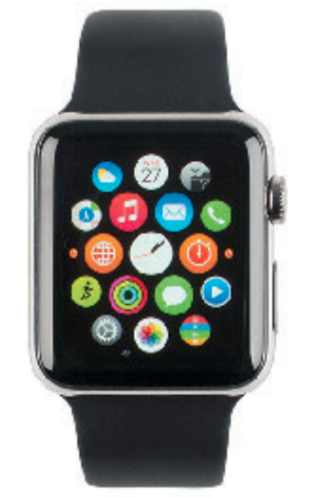
\includegraphics[width=2.5cm]{98_Bilder/06_Smartwatch_Produkte/AppleWatch}
  & 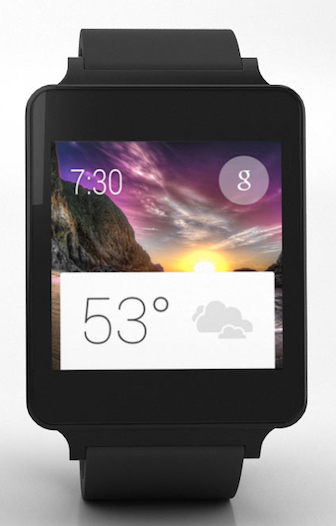
\includegraphics[width=2.5cm]{98_Bilder/06_Smartwatch_Produkte/LGGWatch}
  & 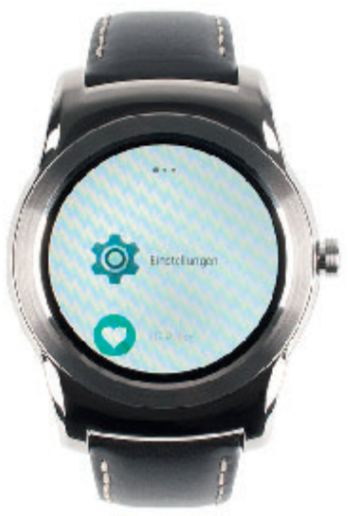
\includegraphics[width=2.5cm]{98_Bilder/06_Smartwatch_Produkte/LGWatchUrbane} \\ \hline
\textbf{Smartwatch}
  & Apple Watch \cite{stwt:sw}
  & LG G Watch
  & LG Watch Urbane \cite{stwt:sw} \\ \hline
\textbf{Betriebsystem}
  & WatchOS
  & Android Wear
  & Android Wear \\ \hline
\textbf{Funktionen}
  & gut
  & befriedigend
  & befriedigend \\ \hline
- Nachrichten
  & empfangen möglich, \newline senden per Sprachnachricht,\newline Emojis senden
  & empfangen möglich, \newline senden per Sprachnachricht
  & empfangen möglich, \newline senden per Sprachnachricht \\ \hline
- Telefonieren
  & führen von Gespräche
  & nur Notifikation
  & nur Notifikation \\ \hline
- Display
  & 42mm 312x390px \newline 38mm 272x340px
  & 1.65 Zoll 280x280px
  & 1.3 Zoll 320x320px \\ \hline
\textbf{$\varnothing$ Akkulaufzeit}
  & 19h
  & 30h
  & 20h \\ \hline
\textbf{Datensendungsverhalten}
  & verschlüsselt
  & verschlüsselt
  & verschlüsselt \\ \hline
\textbf{Smartphone-Betriebssystem}
  & ab iOS 8.2
  & ab Android 4.3 \newline ab iOS 8.2
  & ab Android 4.3 \newline ab iOS 8.2 \\ \hline
\textbf{Pulsmesser}
  & optischer Pulsmesser
  & kein Pulsmesser
  & optischer Pulsmesser \\ \hline
\textbf{Gesamteindruck}
& bestes Display \newline viele Funktionen \newline \textbf{befriedigend - gut}
& Always-On Display \newline befriedigender Akku \newline \textbf{befriedigend}
& rundes Display \newline edle Verarbeitung \newline \textbf{befriedigend} \\ \hline
\end{tabular}
\caption{Technische Daten von Smartwatches - Teil 1}
\end{minipage}
\end{table}

\begin{table}[H]
\begin{minipage}{\textwidth}
\centering
\begin{tabular}{|>{\columncolor[gray]{0.8}}p{4cm}|p{4cm}|p{4cm}|p{4cm}|}
\hline

  & 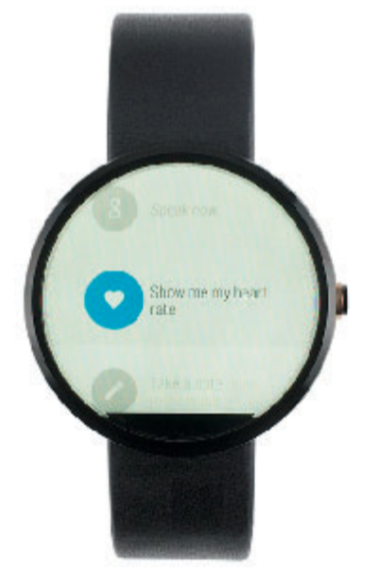
\includegraphics[width=2.5cm]{98_Bilder/06_Smartwatch_Produkte/MotorolaMoto360}
  & 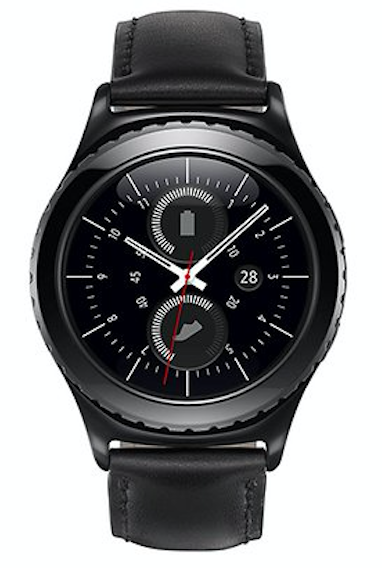
\includegraphics[width=2.5cm]{98_Bilder/06_Smartwatch_Produkte/SamsungGearS2}
  & 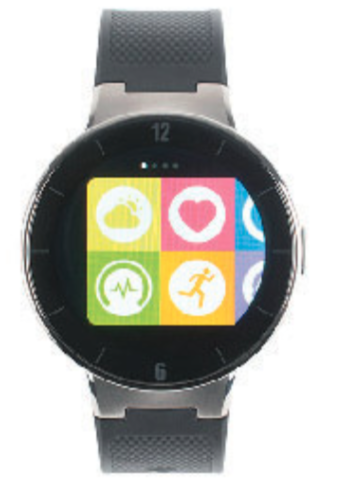
\includegraphics[width=2.5cm]{98_Bilder/06_Smartwatch_Produkte/AlcatelOnetouchWatch} \\ \hline
\textbf{Smartwatch}
  & Motorola Moto 360 \cite{stwt:sw}
  & Samsung Gear S2 \cite{adpt:sss2}
  & Alcatel Onetouch Watch \cite{stwt:sw} \\ \hline
\textbf{Betriebsystem}
  & Android Wear
  & Tizen
  & proprietäres Alcatel OS \\ \hline
\textbf{Funktionen}
  & befriedigend
  & gut
  & befriedigend \\ \hline
- Nachrichten
  & empfangen möglich, \newline senden per Sprachnachricht
  & empfangen möglich, \newline senden möglich
  & empfängt nur Kurznachrichten \\ \hline
- Telefonieren
  & nur Notifikation
  & nur Notifikation \newline bei eSIM Variante möglich
  & nur Notifikation \\ \hline
- Display
  & 1.57 Zoll 360x290px
  & 1.2 Zoll 360x360px
  & 1.3 Zoll 320x320px \\ \hline
\textbf{$\varnothing$ Akkulaufzeit}
  & 10h
  & 38h
  & 20h \\ \hline
\textbf{Datensendungsverhalten}
  & verschlüsselt
  & verschlüsselt
  & unverschlüsselt \\ \hline
\textbf{Smartphone-Betriebssystem}
  & ab iOS 8.2
  & ab Android 4.4
  & ab Android 4.3 \newline ab iOS 7 \\ \hline
\textbf{Pulsmesser}
  & optischer Pulsmesser
  & optischer Pulsmesser
  & optischer Pulsmesser \\ \hline
\textbf{Gesamteindruck}
& bestes Display \newline meiste Funktionen \newline \textbf{befriedigend}
& Intuitive Lünette \newline gute Akkuleistung \newline \textbf{befriedigend - gut}
& schwaches Display \newline mangelhafte Datenübertragung \newline \textbf{mangelhaft} \\ \hline
\end{tabular}
\caption{Technische Daten von Smartwatches - Teil 2}
\end{minipage}
\end{table}

\section{Entscheid Smartwatch}
Wenn nur der Funktionsumfang betrachtet wird, wäre eine Apple Watch oder die Samsung Gear S2 die bevorzugte Wahl gewesen. Die Samsung ist erst seit Oktober 2015 erhältlich, folglich fiel diese, Aufgrund des späten Erscheinungsdatum und dessen Samsung-proprietären Betriebssystem Tizen, aus dem Katalog.

Die Apple Watch wurde nicht gewählt, weil die Apple-Plattform kein offenes System ist. Ein weiterer Entscheidungspunkt ist, dass der Markt de facto aus einem Produkt besteht. Es sei denn, man unterscheidet die Modellvarianten Watch und Watch Sport sowie die Grössen, welche sich nur optisch voneinander abheben.

Ausgewählt wurden zwei Produkte, welche nicht sehr aufgefallen sind. Obwohl sie nicht besonders spektakulär sind, leisten sie genug, um den meisten Bedürfnissen, aus der vorhergehenden Analysen, zu genügen: Die \textbf{LG G Watch} und die \textbf{Motorola Moto 360}.

Als die erste auf dem Markt erhältliche Android Wear Smartwatch, wurde die LG G Watch ausgewählt. Der eingebaute Snapdragon 400 Prozessor rechnet mit 1,2 \gls{GHz}, hat 512\gls{MB} \gls{RAM} und hat einen rechteckigen Bildschirm. Ein Pluspunkt der LG Datenuhr: Sie kann über USB gedebuggt werden. Dies erhöht die Effizienz bei der Entwicklung von Apps.

Um ein Android Wear Vergleichsobjekt zu erhalten, kam die neuere Motorola Moto 360 zusätzlich in die Entscheidung. Diese arbeitet mit einem Texas Instrument OMAP 3 Prozessor mit 1 \gls{GHz}, hat ebenfalls 512\gls{MB} \gls{RAM} und hat einen runden Touchscreen. Mehrwert der Moto 360 zur G Watch ist, ein eingebautes \gls{WLAN}-Modul, Lichtsensor, Pulssensor und eine physische Taste. Bedauerlicherweise kann sie nur über Bluetooth gedebuggt werden, was viel Zeit beansprucht, um entwickelte Apps zu übertragen.

Ein wichtiger Unterschied beider Geräte ist der Bildschirmmodus. Die G Watch erlaubt den Always-On Betrieb, was einer App erlaubt das Display während der Laufzeit immer eingeschaltet zu lassen. Die Moto 360 hingegen hat den Ambient Mode, welcher den Bildschirm abdunkelt, die App jedoch am laufen hält. Hierbei ist zu erwähnen, dass Android Wear Apps sich schliessen, wenn der Bildschirm in den Ruhezustand geht.

Durch die Entscheidung für Android Wear liegt der Schwerpunkt der Entwicklung auf Java sowie das Layouting auf \gls{XML}. Die Entwicklungsumgebung konnte auch auf Android Studio eingeschränkt werden, da im Sommer 2015 bekannt gegeben wurde, dass die Entwicklung des Eclipse Plugin eingestellt wird (vgl. \cite{adbl:eadt}). Eine alternative Entwicklungsumgebung, welche die Effizienz eines Android Studios hat oder bedeutende Vorteile hat, ist keine aufgefallen.
